\section{Debug chat terminal} \label{sec:debugProgram}
Om het netwerk te ontwikkelen is het handig om een manier te hebben om het systeem te kunnen debuggen. Hiervoor is een debug chat terminal geschreven. Dit programma draait op een XMega en werkt via een seriële verbinding met een computer over USB. De terminal kan gebruikt worden in een programma zoals TeraTerm/Minicom. In \autoref{fig:debugTerminal} is de terminal te zien. Wanneer de gebruiker iets typt, wordt dit op het scherm getoond, net als in een normale command line. Wanneer er een bericht binnenkomt, wordt deze naar de terminal geprint, zonder de gebruikersinvoer te onderbreken. De gebruiker kan berichten sturen door deze te typen en vervolgens op enter te drukken. Er zijn ook een aantal commando's die de gebruiker kan uitvoeren. Deze commando's beginnen met een slash (/), zodat ze niet worden verward met berichten die verstuurd moeten worden.
De beschikbare commando's zijn:

\begin{description}
    \item[/help] Print een lijst van alle beschikbare commando's, en hoe deze gebruikt moeten worden.

    \item[/dest] Verander het bestemmings-ID van berichten.

    \item[/list] Print de huidige lijst van vriendjes. 

    \item[/send] Verstuur een bericht. Dit commando wordt zelden gebruikt, doordat een bericht ook verstuurd kan worden door het in de terminal te typen en op enter te drukken. /send kan echter wel nuttig zijn voor het versturen van berichten die beginnen met een slash.

    \item[/myid] Print het ID van de node.

    \item[/keys] Print de twee encryptie keys.

    \item[/key1] Verander encryptie key 1.
    \item[/key2] Verander encryptie key 2. 

    \item[/chan] Verander het NRF kanaal. 
\end{description}


Wanneer op enter gedrukt wordt zonder iets in te vullen wordt het vorige commando uitgevoerd. Dit is erg handig voor het /list commando, aangezien de lijst dan makkelijk herhaaldelijk geprint kan worden. Ook is het nuttig voor het testen van verbindingen. Berichten kunnen snel herhaald worden door steeds op enter te blijven drukken. Wanneer de node iets ontvangt, wordt dit in de terminal als hexadecimale geprint, en als ASCII karakter, als deze bestaat. 

\begin{figure}[ht]
    \centering
    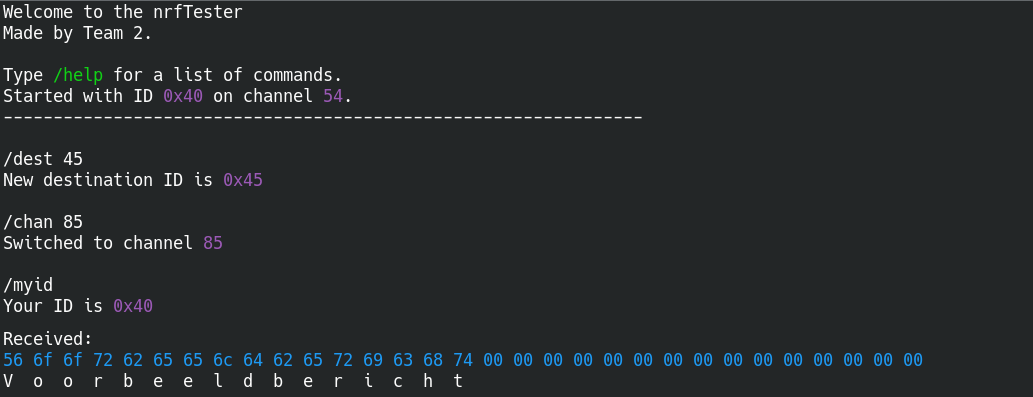
\includegraphics[width=0.8\textwidth]{img/nrfchat.png}
    \caption{Hoe de debug chat terminal eruit ziet.}
    \label{fig:debugTerminal}
\end{figure}


% Het NrfChat programma laat mensen met elkaar praten via een CLI interface. Om het programma in te stellen kunnen een aantal commando's

% \subsubsection{Commands}
% De commando's die in het nrfChat programma kunnen worden gebruikt.

% \begin{table}[h]
%     \begin{tabular}{|l|l|} \hline
%         \textbf{Commando} & \textbf{Beschrijving} \\\hline
%         help & Laat een hulp bericht zien \\\hline
%         chan & Selecteer het kanaal waarop wordt gezonden en ontvangen\\\hline
%         send & Stuur een bericht \\\hline
%         list & Laat de vriendjes lijst zien\\\hline
%         dest & Stel doel ID in voor berichten die met send worden verstuurd \\\hline
%         myid & Laat zien wat het ID is van de node \\\hline
%         keys & Laat zien wat de keys zijn \\\hline
%         key1 & Definieert key 1 met wat erachter wordt gezet\\\hline
%         key2 & Definieert key 2 met wat erachter wordt gezet\\\hline
%     \end{tabular}
% \end{table}

% \subsubsection{Functionele blokken}

% \subsubsection{nrfChat}
%     \section{Debug nodes}
Het nrfChat bestand is bedoeld om op een gebruikersvriendelijke manier met andere nodes te communiceren. Het programma laat de terminal in principe functioneren als command line, waar commando's in getypt kunnen worden om uit te voeren. Het is niet bedoeld als een sensormodule, maar in plaats daarvan als een nuttige debugging terminal voor engineers.

De gebruiker kan commando's invoeren, beginnende met een slash, die onder andere gebruikt kunnen worden om de bestemming van berichten in te stellen, of de huidige burenlijst/vriendjeslijst uit te printen. Alles wat in de terminal getypt wordt dat niet begint met een slash, wordt gezien als een bericht om verstuurd te worden. Deze berichten worden via iso.c verstuurd naar de geselecteerde ontvanger.

\paragraph*{Init}
Bij het initialiseren van nrfChat worden de volgende acties ondernomen:
\begin{enumerate}
    \item iso.c wordt geïnitialiseerd. 
    \item De ontvangst callback functie van iso.c wordt ingesteld op de ontvangst functie (zie \autoref{ch:messageReceive}).
    \item De gebruikersinput callback functie van terminal.c ingesteld op de input interpreteer functie (zie \autoref{ch:interpreter}).
    \item Er wordt een header geprint met een welkomstbericht met een instructie om /help in te voeren, en het ID en kanaal van de node.
\end{enumerate}

Hierna kan de gebruiker commando's en berichten typen.

\paragraph*{Loop}
In de loop worden ingevoerde karakters doorgegeven aan terminal.c. Ook wordt \texttt{isoUpdate} aangeroepen. Zie \autoref{lst:nrfChatLoop}.

\begin{lstlisting}[caption={De nrfChat loop},captionpos=b,label={lst:nrfChatLoop},style=c,xleftmargin=.\textwidth,xrightmargin=.\textwidth]
void nrfChatLoop(void) {
    while (1) {
        // Get the character from the user.
        // Use char instead of uint16_t,
        // because we don't need to handle any '\0's.
        char newInputChar = uartF0_getc();

        if(newInputChar != '\0') {
           terminalInterpretChar(newInputChar);
        }

        isoUpdate();
    }
}
\end{lstlisting}

\paragraph*{Berichten ontvangen} \label{ch:messageReceive}
Ontvangen berichten worden direct doorgestuurd naar de \texttt{terminalPrintStrex} functie van terminal.c. Zie \autoref{ch:printStrex}.

\paragraph*{Interpreteer input} \label{ch:interpreter}

De input wordt in meerdere stappen geïnterpreteerd. De interpreteer functie krijgt de ingevoerde regel tekst mee als argument, en wordt uitgevoerd wanneer er op enter wordt gedrukt door de gebruiker.
Het eerste deel van de functie is te zien in \autoref{lst:interpretInputStart}. Hier kijkt de functie eerst of de input begint met een slash. Als dit niet het geval is, wordt de volledige input direct verstuurd naar de geselecteerde bestemming. Wanneer de input wel met een slash begint, wordt de pointer naar de input met 1 verhoogt, zodat de rest van de code geen rekening meer hoeft te houden met deze slash.

\begin{lstlisting}[caption={Eerste deel van de interpreter},captionpos=b,label={lst:interpretInputStart},style=c,xleftmargin=.\textwidth,xrightmargin=.\textwidth]
// If no '/' is given, just send the inputted string.
if(input[0] != '/') {
    send(input);
    return;
}

// If a '/' is given, we want to interpret from the character after it.
input++;
\end{lstlisting}

Er worden vervolgens twee constante en statische arrays aangemaakt (zie \autoref{lst:interpretInputFPointers}). Eén van de arrays bevat al de commando's die uitgevoerd kunnen worden door de gebruiker. De andere array bevat de functie pointers naar de corresponderende functies.
Aangezien de functienamen op de zelfde index zitten als de functie pointers, kunnen de arrays gebruikt worden als look-up table.

\begin{lstlisting}[caption={De look-up table van de interpreter},captionpos=b,label={lst:interpretInputFPointers},style=c,xleftmargin=.\textwidth,xrightmargin=.\textwidth]
// Make a corresponding array of 4 letter function names.
static const char commands[COMMANDS][4] = {
    "send", "help", "chan", "list", "dest", "myid", "keys", "key1", "key2"
};
// Make an array of functions.
static const void (*functions[COMMANDS])(char*) = {
    send, help, chan, list, dest, myid, keys, key1, key2
};
\end{lstlisting}

De code gaat vervolgens langs elk van de functienamen. Wanneer het ingevoerde commando gelijk is aan een van de functienamen in de \texttt{commands} array, wordt de functie op dezelfde index uit de \texttt{functions} array uitgevoerd. De functie krijgt de input pointer mee als argument, waar 5 bij op wordt geteld. Dit is zodat de functie alleen het begin van de argumenten van het commando meekrijgt.

Wanneer de gebruiker echter maar 5 karakters heeft ingevoerd (Zoals \texttt{/dest}), lopen we tegen een probleem aan. De pointer die de functie meekrijgt ligt dan namelijk in de gebruikersinput buffer, \textit{na} de \textbackslash0 die wordt toegevoegd. Hierdoor weet de functie niet waar het einde van de gebruikersinput is, en kunnen er geheugenproblemen ontstaan. Dit is opgelost door een extra \textbackslash0 in de buffer te zetten wanneer de invoer maar 5 karakters lang is. Zo wordt aan de functie een pointer meegegeven naar een \textbackslash0, zodat deze kan weten dat de gebruiker geen verdere argumenten heeft meegegeven.

\begin{lstlisting}[caption={De code die het ingevoerde commando als functie uitvoert},captionpos=b,label={lst:interpretInputRun},style=c,xleftmargin=.\textwidth,xrightmargin=.\textwidth]
for(uint8_t i = 0; i < COMMANDS; i++) {
    if(strncmp(commands[i], input, 4) == 0) {
        // Prevent problems relating to inputs with no arguments.
        if(input[4] == '\0') input[5] = '\0';

        // Run the command, with the text after it as argument.
        functions[i](input + 5);
        return;
    }
}
printf("I don't know that command :(\n");
\end{lstlisting}



\paragraph*{Help}
Help print een gebruikersaanwijzing uit voor de gebruiker, als een lijst van alle commando's en hun functionaliteit.

\paragraph*{Chan}
Chan is een erg simpel commando. Het enige wat het doet is de frequentie veranderen waar de nrf chip op zendt en ontvangt. De werking van de functie is te zien in \autoref{lst:chan}.
\begin{lstlisting}[caption={De chan functie},captionpos=b,label={lst:chan},style=c,xleftmargin=.\textwidth,xrightmargin=.\textwidth]
void chan(char *arguments) {
    uint8_t channel = atoi(arguments);

    nrfStopListening();
    nrfSetChannel(channel);
    nrfStartListening();

    printf("\nSwitched to channel %d\n\n", channel);
}
\end{lstlisting}

De functie heeft geen afhandeling van een ongeldige input. Dit is omdat \texttt{atoi} altijd een 0 teruggeeft wanneer hij tegen een probleem aanloopt bij het parsen van een getal. Hierdoor wordt het kanaal gewoon naar 0 gezet wanneer de gebruiker een ongeldige invoer geeft. Hier wordt de gebruiker ook van op de hoogte gesteld, door de \texttt{printf} mededeling. Aangezien de kanaalfrequentie wordt berekent door middel van \autoref{eq:frequentie} is 0 gewoon een geldige kanaalfrequentie, en hoeft er geen actie ondernomen worden. Deze functie is in principe alleen bedoelt voor debugging doeleinden, aangezien de kanaalfrequentie al in de ISO is vastgesteld als 38 (2438 MHz).

\begin{equation} \label{eq:frequentie}
    f = 2400 + \textrm{kanaal [MHZ]})
\end{equation}

\paragraph*{Dest}
De dest functie werkt in principe hetzelfde als chan. Het enige verschil is dat dest het opgeslagen bestemmings-ID verandert in plaats van de frequentie. In \autoref{lst:dest} is te zien dat de dest functie wel ongeldige input afhandelt. Dit is omdat, waar 0 een geldige frequentie is bij /chan, het geen geldig ID is volgens de ISO. Het ID wordt uitgelezen met \texttt{strtol}, welke een hexadecimale string in een integer omzet. Dit is omdat ID's altijd als hexadecimaal getal genoteerd worden.

\begin{lstlisting}[caption={De dest functie},captionpos=b,label={lst:dest},style=c,xleftmargin=.\textwidth,xrightmargin=.\textwidth]
void dest(char *arguments) {
    if(arguments[0] == '\0') {
        printf("Usage:" COMMAND_COLOR " /dest" NO_COLOR " <ID>\n\n");
        return;
    }

    uint8_t newId = strtol(arguments, NULL, 16);
    if(newId == 0) printf(ERROR_COLOR "Invalid ID entered.\n\n" NO_COLOR);
    else {
        destinationId = newId;
        printf("New destination ID is " ID_COLOR "0x%02x" NO_COLOR "\n\n", newId);
    }
}
\end{lstlisting}


\paragraph*{Send}
De send functie stuurt encrypted alles wat er meegegeven wordt op via de \texttt{isoSendPacket} functie, zoals te zien in \autoref{lst:send}
\begin{lstlisting}[caption={De send functie},captionpos=b,label={lst:send},style=c,xleftmargin=.\textwidth,xrightmargin=.\textwidth]
void send(char *command) {
    // Set the rest of the inputbuffer to zero so that we don't accidentally 
    send previous messages with the message.
    uint8_t argLength = strlen(arguments);
    memset(arguments + argLength, 0, PAYLOAD_SIZE - argLength);

    uint8_t *data = keysEncrypt((uint8_t*)arguments, PAYLOAD_SIZE, key1Data, 
    strlen(key1Data), key2Data, strlen(key2Data));
    if(isoSendPacket(destinationId, (uint8_t*) data, PAYLOAD_SIZE)) 
        printf("Failed to send message\n");      
}
\end{lstlisting}


\paragraph*{List}
Het enige wat de list functie doet is de \texttt{printFriends} functie uitvoeren, te vinden in \autoref{ch:printFriends}.


\paragraph*{MyID}
MyID print het ID van de node naar de terminal. Dit is erg nuttig wanneer de geprinte header niet meer zichtbaar is door bijvoorbeeld een groot aantal ontvangen berichten.

\paragraph*{Keys}
Keys print key1 en key2 naar de terminal. Dit is erg nuttig wanneer het niet meer duidelijk was welke keys er werden gebruikt. Deze staan in Hexadecimaal inplaats van ASCII zodat de gebruiker nog een beetje moet ontcijferen wat de key ookalweer was.

\paragraph*{Key1}
Dit commando zet aan de array key1 de ASCII waarde van wat in de terminal is ingevoerd. 

\paragraph*{Key2}
Dit commando is hetzelfde als key1, maar doet dit dan voor key2.

% \subsubsection{Terminal}
%     
Terminal.c is een library die gemaakt is voor nrfChat.c, maar ook voor andere debugging doeleinden. De library is gemaakt omdat, wanneer er iets op de terminal uitgeprint wordt, dit dwars door de huidige input heengaat van de gebruiker. De input staat nog steeds in de buffer, en kan nog steeds uitgevoerd worden, hij is alleen niet meer leesbaar. Dit beloofde uiteindelijk frustrerend genoeg om snel een library te schrijven die gebruikt kan worden om zowel debug informatie als ontvangen berichten uit te printen. Ook regelt de library het bufferen van alle gebruikersinput.

\subsubsection{Intrepeteer input}
Aangezien programma's zoals Minicom, TeraTerm en PuTTY elk getypte karakter direct naar de microcontroller sturen, moeten we onze eigen linebuffer bijhouden. Hier is de functie \texttt{terminalInterpretChar} voor bedoelt. Deze functie moet elke keer aangeroepen worden wanneer de gebruiker een toets op het toetsenbord intikt. De functie zet dan het getypte karakter dan in een buffer. 

Doordat backspaces niet behandelt worden door een linebuffer van de terminal, zoals normaal bij C programma's, moeten we deze zelf afhandelen. In \autoref{lst:backspaces} is te zien hoe dit gebeurt. De buffer index wordt met 1 vermindert, en in de terminal wordt het vorige karakter vervangen door een spatie.



\begin{lstlisting}[caption={Backspaces afhandelen},captionpos=b,label={lst:backspaces},style=c,xleftmargin=.\textwidth,xrightmargin=.\textwidth]
    // Handle backspaces.
    if(inChar == '\b' && inputBufferIndex) {
        // Go back 1, make the char empty, and go back again.
        // If we only print \b the cursor would simply move
    // to the left without removing any characters.
    printf("\b \b");
    inputBufferIndex--;
    return;
}
\end{lstlisting}

\subsubsection{Command callback}
Wanneer het programma een return karakter (\textbackslash~n) tegenkomt, moet het ingevoerde commando uitgevoerd worden. Dit wordt gedaan door middel van een callback functie. De callback functie kan worden ingesteld met een initialisatie functie. De 

\subsubsection{Print string}
\subsubsection{Print hex}
\subsubsection{Print string en hex} \label{ch:printStrex}

    

    